\documentclass[11pt]{article}
\usepackage{geometry, titlesec}
\usepackage[parfill]{parskip}
\usepackage[italicdiff]{physics}
\usepackage{amsfonts, amsthm}
\usepackage[cm]{fullpage}
\usepackage{fancyhdr}
\usepackage{enumitem}
\usepackage{xcolor, soul}
\usepackage{graphicx}
\usepackage[export]{adjustbox}
\usepackage{siunitx}
%\allowdisplaybreaks

\renewcommand{\thesubsection}{\thesection.\alph{subsection}}
\setenumerate[1]{label={(\alph*)}}

\makeatletter
\renewcommand*\env@cases[1][1.2]{%
  \let\@ifnextchar\new@ifnextchar
  \left\lbrace
  \def\arraystretch{#1}%
  \array{@{}l@{\quad}l@{}}%
}
\makeatother
 
\renewcommand{\footrulewidth}{.2pt}
%\setlist[enumerate]{leftmargin=*}
\pagestyle{fancy}
\fancyhf{}
\lhead{Physics 132-B}
\chead{\textbf{Discussion 4 Solutions}}
\rhead{A--De Discussion}
\setlength{\headheight}{11pt}
\setlength{\headsep}{11pt}
\setlength{\footskip}{24pt}
\lfoot{\today}
\rfoot{\thepage}

\titleformat{\subsection}[runin]{\normalfont\large\bfseries}{\thesubsection}{1em}{}
\newcommand{\refeq}[1]{(\ref{#1})}

\newcommand{\beq}{\begin{equation*}}
\newcommand{\eeq}{\end{equation*}}

\newcommand{\beqn}{\begin{equation}}
\newcommand{\eeqn}{\end{equation}}

\newcommand{\blg}{\begin{align*}}
\newcommand{\elg}{\end{align*}}


\newenvironment{statement}
{
%    \color{gray}
    \ignorespaces
}
{
%    \smallskip
}

\newenvironment{problem}
{
    \color{darkgray}
    \ignorespaces
}

\newenvironment{solution}
{
    \paragraph{Solution}
    \ignorespaces
}
{
    \bigskip
}

\renewcommand{\vec}[1]{\mathbf{#1}}


\begin{document}
	

\newcommand{\vE}{\vec{E}}
\newcommand{\vEq}{\vE_1}
\newcommand{\vEw}{\vE_2}
\renewcommand{\qq}{q_1}
\newcommand{\qw}{q_2}
\newcommand{\tht}{\theta}
\newcommand{\thtq}{\tht_1}
\newcommand{\thtw}{\tht_2}
\newcommand{\Eq}{E_1}
\newcommand{\Ew}{E_2}
\newcommand{\Ex}{E_x}
\newcommand{\Ey}{E_y}
\newcommand{\ent}{\epsilon_0}
\newcommand{\fk}{\frac{1}{4\pi\ent}}

\begin{minipage}[l]{0.65\textwidth}
\paragraph{Problem 21.96}
%\paragraph{Problem 1}
\begin{problem}
	Two charges are placed as shown in Fig.~P21.96.  The magnitude of $\qq$ is \SI{3.00}{\micro\coulomb}, but its sign and the value of the charge $\qw$ are not known.  The direction of the net electric field $\vE$ at point $P$ is entirely in the negative $y$ direction. \medskip
	\begin{enumerate}
		\item Considering the different possible signs of $\qq$ and $\qw$, four possible diagrams could represent the electric fields $\vEq$ and $\vEw$ produced by $\qq$ and $\qw$.  Sketch the four possible electric field configurations. \medskip
		\item Using the sketches from part (a) and the direction of $\vE$, deduce the signs of $\qq$ and $\qw$. \medskip
		\item Determine the magnitude of $\vE$.
	\end{enumerate}
\end{problem}
\end{minipage}%
\hspace{0.05\textwidth}%
\begin{minipage}[r]{0.3\textwidth}
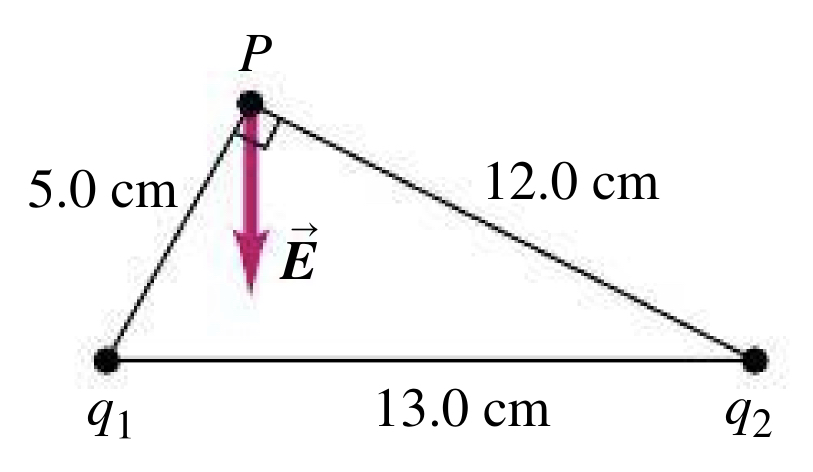
\includegraphics[width=\textwidth]{P21-96.jpeg}
\center \textbf{Figure P21.96}
\end{minipage}

\begin{solution}
	\begin{enumerate}
		\item The four possible diagrams are:
		
		\begin{center}
			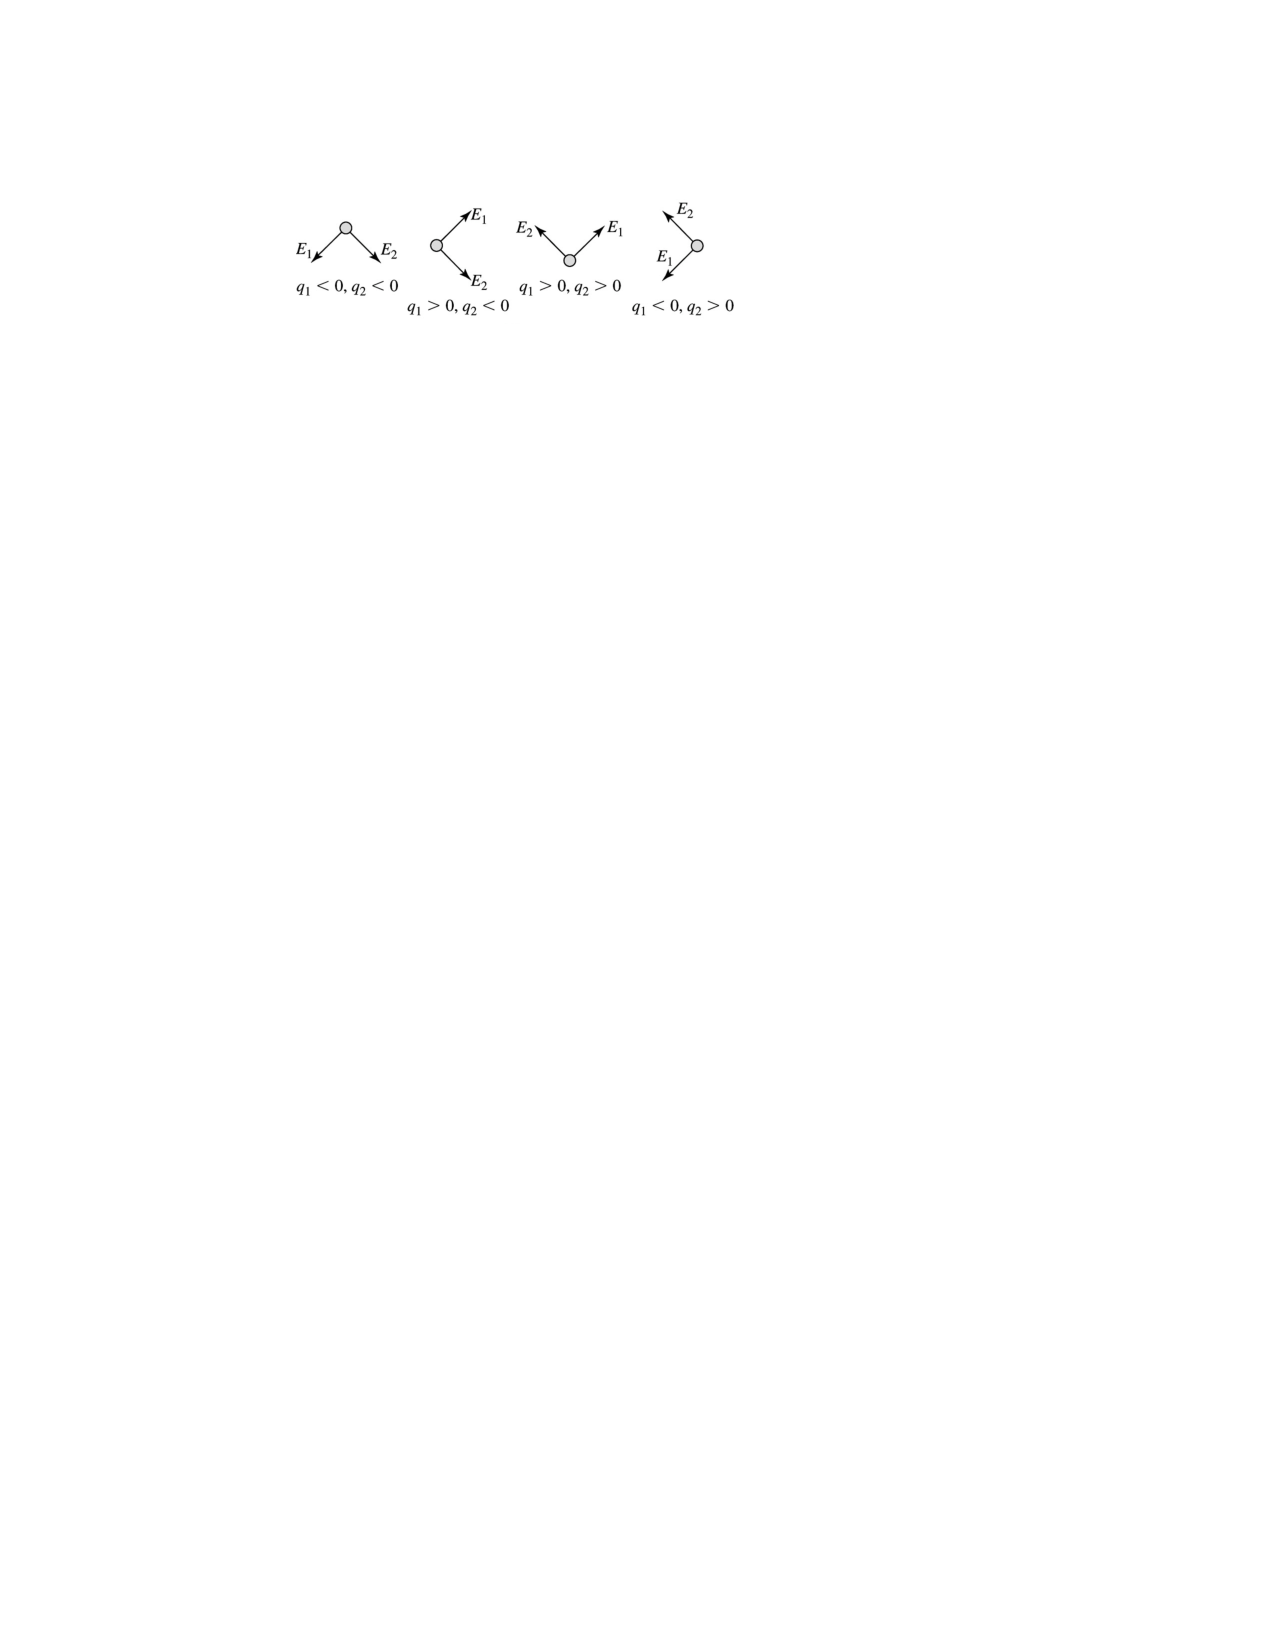
\includegraphics[scale=1.5]{P21-96a}
		\end{center}
		
		Here $E_1$ and $E_2$ indicate the electric fields of $\qq$ and $\qw$, respectively.
		
		\item The first diagram is the only one that has the net $\vE = \vEq + \vEw$ pointing in the $-y$ direction like we want.  This means both $\qq$ and $\qw$ are negative.  (We also could have deduced this by placing a positive test charge at $P$, and realizing we need $\qq$ and $\qw$ to be negative in order to produce an electric field pointing down.)
		
		\item Using the expression for the electric field due to a point charge, we can find the magnitudes of $\Eq$ and $\Ew$:
		\begin{align*}
			\Eq &= \fk \frac{\abs{\qq}}{(\SI{5.0}{\cm})^2} = -\fk \frac{\SI{3.00}{\micro\coulomb}}{(\SI{5.0}{\cm})^2}, &
			\Ew &= \fk \frac{\abs{\qw}}{(\SI{12.0}{\cm})^2}.
		\end{align*}
		Notice that we need to solve for $\qw$, which we can do by force balance.  We need to find and add the $x$ and $y$ components of $\vEq$ and $\vEw$, which we can do by finding their angles from the horizontal.  Call these angles $\thtq$ and $\thtw$.  Building off of our diagram for (a), we can make something similar to a force diagram, but for the electric field:
		
		\begin{center}
			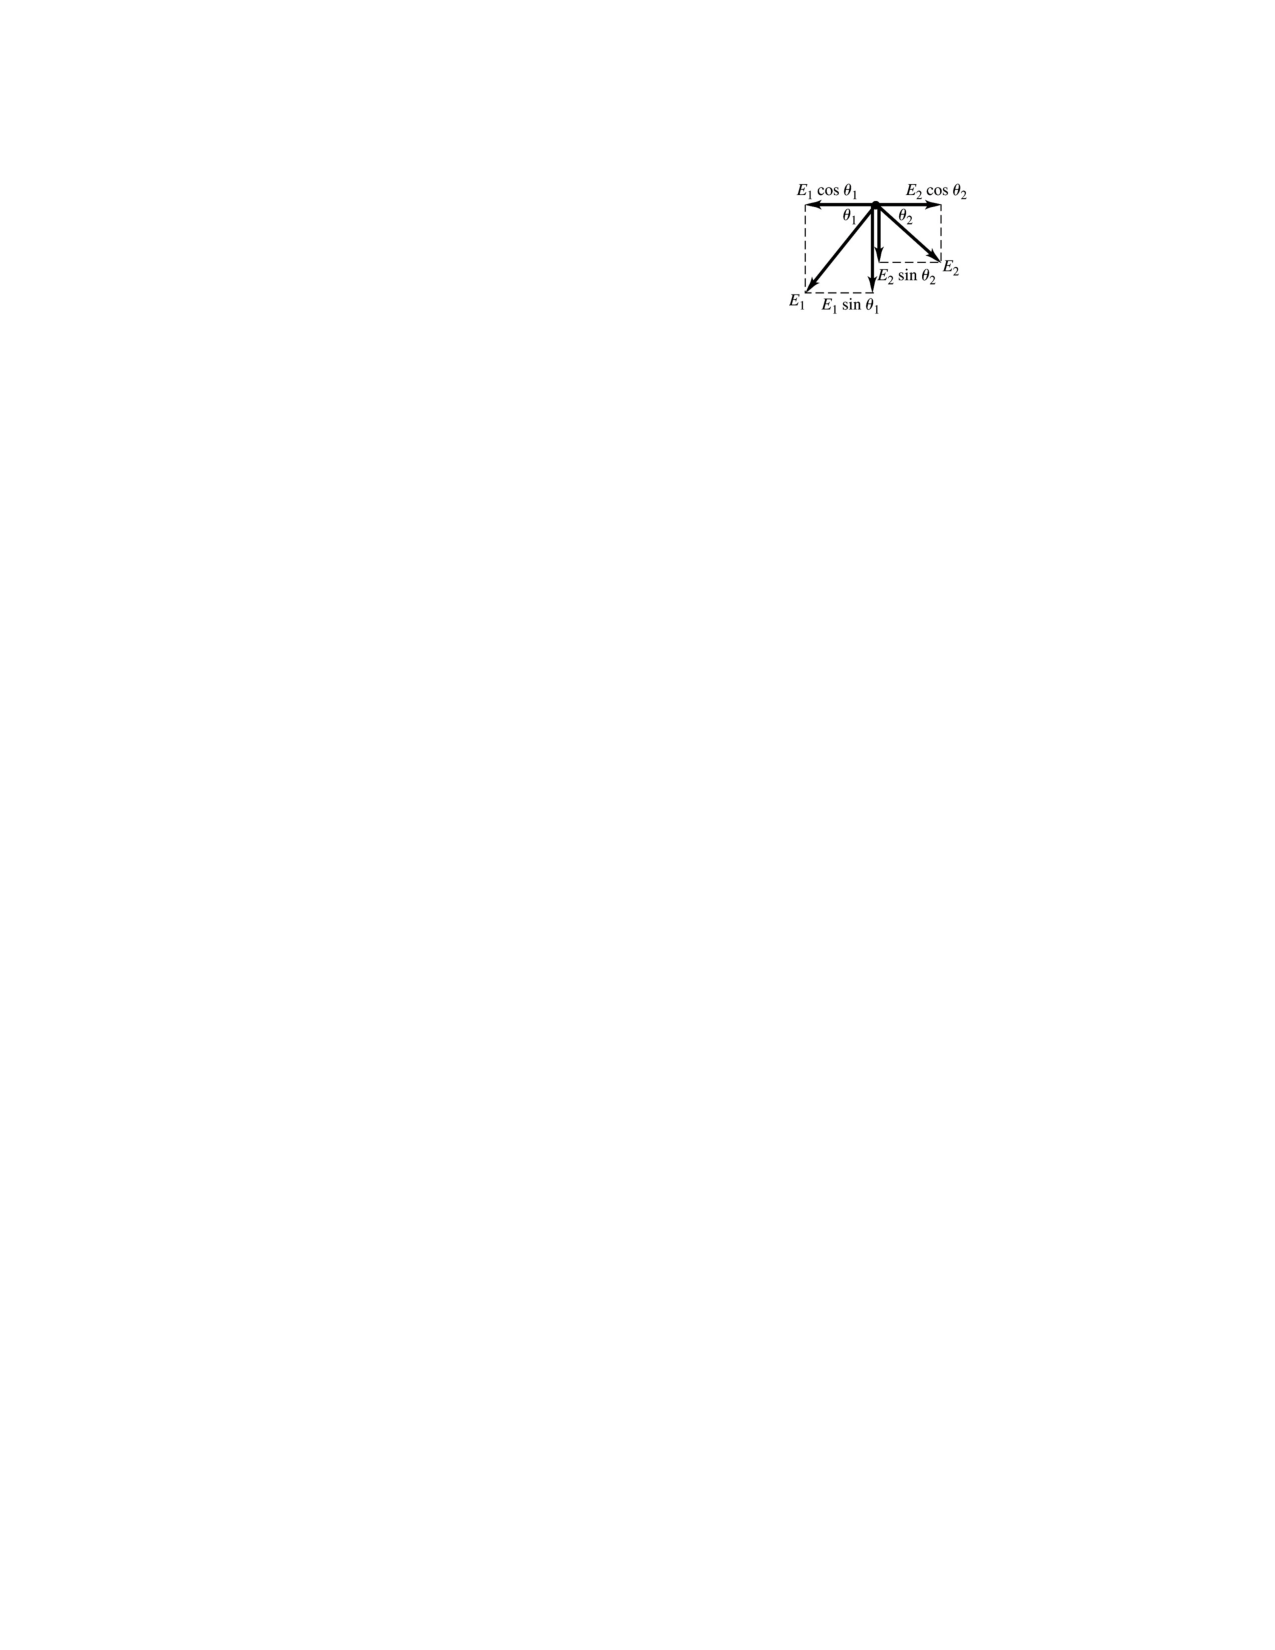
\includegraphics[scale=1.5]{P21-96b}
		\end{center}
		
		From Fig.~P21.96, we can write down
		\begin{align*}
			\cos\thtq &= \frac{5}{13}, &
			\sin\thtq &= \frac{12}{13}, &
			\cos\thtw &= \frac{12}{13}, &
			\sin\thtw &= \frac{5}{12}.
		\end{align*}
		
		First, let's balance forces in the $x$ direction, in which we know there's 0 net electric field.  This will allow us to find the magnitude of $\qw$:
		\beq
			0 = \Ex
			= {\Eq}_x + {\Ew}_x
			= \Eq \cos\thtq + \Ew \cos\thtw
			= -\frac{5}{13} \fk \frac{\SI{3.00}{\micro\coulomb}}{(\SI{5.0}{\cm})^2} + \frac{12}{13} \fk \frac{\abs{\qw}}{(\SI{12.0}{\cm})^2}
		\eeq
		\beq
			\implies \frac{\SI{3.00}{\micro\coulomb}}{\SI{5.0}{\square\cm}} = \frac{\abs{\qw}}{\SI{12.0}{\square\cm}}
			\implies \abs{\qw} = \frac{36}{5} \si{\micro\coulomb} = \SI{7.2}{\micro\coulomb}.
		\eeq
		Now we can add the forces in the $y$ direction to find the magnitude of $\vE$:
		\begin{align*}
			|\vE| &= \Ey
			= {\Eq}_y + {\Ew}_y
			= \Eq \sin\thtq + \Ew \sin\thtw
			= \frac{12}{13} \fk \frac{\SI{3.00}{\micro\coulomb}}{(\SI{5.0}{\cm})^2} + \frac{5}{12} \fk \frac{\SI{7.2}{\micro\coulomb}}{(\SI{12.0}{\cm})^2} \\
			&= \fk \left( \frac{12}{13} \frac{\SI{3.00e-6}{\coulomb}}{\SI{25e-4}{\square\m}} + \frac{5}{12} \frac{\SI{7.2e-6}{\coulomb}}{\SI{144e-4}{\square\m}} \right)
			= \fk \left( \frac{36}{325} + \frac{36}{1728} \right) \times\SI{e-2}{\coulomb\per\square\meter} \\
			&= (\SI{8.99e9}{\newton\square\meter\per\square\coulomb}) (\SI{0.131e-2}{\coulomb\per\square\meter}) \\
			&= \SI{1.18e7}{\newton\per\coulomb}.
		\end{align*}
	\end{enumerate}
\end{solution}

%\vfill

\newcommand{\dQ}{\dd{Q}}
\newcommand{\dz}{\dd{z}}
\newcommand{\du}{\dd{u}}
\newcommand{\dtht}{\dd{\tht}}
	
\paragraph{Problem 23.82}
%\paragraph{Problem 2}
\begin{problem}
	A hollow, thin-walled insulating cylinder of radius $R$ and length $L$ (like the cardboard tube in a roll of toilet paper) has charge $Q$ uniformly distributed over its surface.
	
	\begin{enumerate}
		\item Calculate the electric potential at all points along the axis of the tube.  Take the origin to be at the center of the tube, and take the potential to be zero at infinity.
		\setcounter{enumi}{2}
		\item Use the result of part (a) to find the electric field at all points along the axis of the tube.
	\end{enumerate}
\end{problem}

\begin{solution}
	\begin{enumerate}
		\item We can think of the tube as being made of a stack of charged rings.  Example~23.11 in the textbook derives the expression for the electric potential due to a ring, which is
			\beq
				V_\text{ring} = \fk \frac{Q_\text{ring}}{\sqrt{x^2 + a^2}},
			\eeq
			where $Q_\text{ring}$ is the total charge of the ring, $x$ is the distance from the center of the ring along its axis, and $a$ is the ring's radius~(Fig.~23.20).
			
%			\includegraphics{P23-20}

			Let the ring have charge $\dQ$ and be at position $z$ along the $x$ axis.  We will need to integrate $z$ from $-L/2$ to $L/2$.  The infinitesimal charge $\dQ$ of the ring is related to the entire charge of the tube through their respective lengths:
			\beq
				\frac{\dQ}{\dz} = \frac{Q}{L} \implies \dQ = \frac{Q}{L} \dz.
			\eeq
			Our integral is then
			\beq
				V = \int_{-L/2}^{L/2} \fk \frac{\dQ}{\sqrt{(x-z)^2 + R^2}}
				= \fk \frac{Q}{L} \int_{-L/2}^{L/2} \frac{\dz}{\sqrt{(x-z)^2 + R^2}}.
			\eeq
			The denominator of the integrand looks kind of gross, so we probably want to do a $u$ substitution.  Let $u = x - z$, so $\du = -\dz$.  Then our integral becomes
			\beq
				V = -\fk \frac{Q}{L} \int_{x + L/2}^{x - L/2} \frac{\du}{\sqrt{u^2 + R^2}}
				= \fk \frac{Q}{L} \int_{x - L/2}^{x + L/2} \frac{\du}{\sqrt{u^2 + R^2}},
			\eeq
			which is possible to do, but we would have to look it up in a table of integrals, and the form is really gross (look it up and see).  Let's try to find an easier way, by finding the electric field first instead of second.
			
			The electric field due to a ring of charge was found in Ex.~21.9:
			\beq
				E_\text{ring} = \fk \frac{Q_\text{ring} x}{(x^2 + a^2)^{3/2}}.
			\eeq
			Setting up the integral over the length of the tube as we did before, we get
			\beq
				E = \int_{-L/2}^{L/2} \fk \frac{\dQ}{[(x-z)^2 + R^2]^{3/2}}
				= \fk \frac{Q}{L} \int_{-L/2}^{L/2} \frac{\dz}{[(x-z)^2 + R^2]^{3/2}}
				= \fk \frac{Q}{L} \int_{x - L/2}^{x + L/2} \frac{\du}{(u^2 + R^2)^{3/2}}.
			\eeq
			
%			and it's best to consult a table of integrals for this one.  We have
%			\begin{align*}
%				V &= \fk \frac{Q}{L} \left[ \ln\left| u + \sqrt{u^2 + R^2} \right| \right]_{x - L/2}^{x + L/2} \\
%				&= \fk \frac{Q}{L} \left( \ln\left| x + \frac{L}{2} + \sqrt{(x + L/2)^2 + R^2} \right| - \ln\left| x - \frac{L}{2} + \sqrt{(x - L/2)^2 + R^2} \right| \right)
%			\end{align*}
%			which we can solve using a trig substitution.  Let $u = R \tan\tht$, so $\du = R \sec^2\tht \dtht$.  The the bounds of integration become
%			\begin{align*}
%				\thtq &\equiv \tan[-1](\frac{x - L/2}{R}), &
%				\thtw &\equiv \tan[-1](\frac{x + L/2}{R}).
%			\end{align*}
%			Using the identity $\tan^2\tht + 1 = \sec^2\tht$, our integral becomes
%			\begin{align*}
%				V &= \fk \frac{Q}{L} \int_{\thtq}^{\thtw} \frac{R \sec^2\tht}{\sqrt{R^2 \tan^2\tht + R^2}} \dtht
%				= \fk \frac{Q}{L} \int_{\thtq}^{\thtw} \frac{\sec^2\tht}{\sqrt{\tan^2\tht + 1}} \dtht
%				= \fk \frac{Q}{L} \int_{\thtq}^{\thtw} \sec\tht \dtht \\
%				&= \fk \frac{Q}{L} \int_{\thtq}^{\thtw} \frac{1}{\cos\tht} \dtht
%				= \ln(\sec\tht + \tan\tht)
%			\end{align*}
	\end{enumerate}
\end{solution}


\clearpage

\begin{minipage}[b]{0.65\textwidth}
\paragraph{Problem 22.32}
%\paragraph{Problem 3}
\begin{problem}
	A cube has sides of length $L = \SI{0.300}{\meter}$.  One corner is at the origin~(Fig.~E22.6).  The nonuniform electric field is given by ${\vE = (\SI{-5.00}{\newton\per\coulomb\per\meter})x \, \vec{\hat{i}} + (\SI{23.00}{\newton\per\coulomb\per\meter}) z \, \vec{\hat{k}}}$. \medskip
	\begin{enumerate}
		\item Find the electric flux through each of the six cube faces $S_1,\ S_2,\ S_3,\ S_4,\ S_5$, and $S_6$. \medskip
		\item Find the total electric charge inside the cube.
	\end{enumerate}
\end{problem}
\end{minipage}%
\hspace{0.05\textwidth}%
\begin{minipage}{0.3\textwidth}
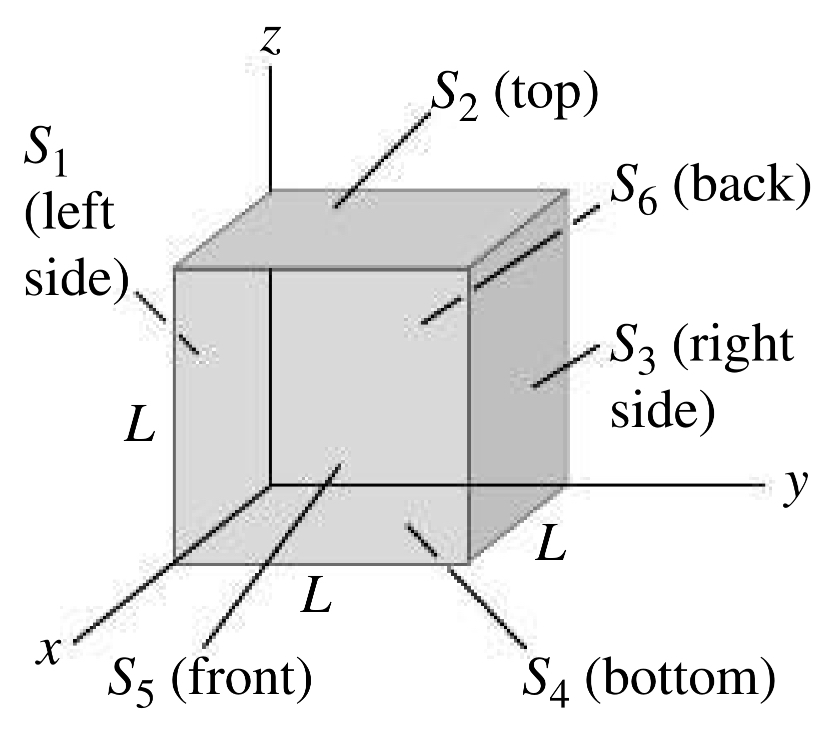
\includegraphics[width=\textwidth]{E22-6.jpeg}
\center \textbf{Figure E22.6}
\end{minipage}

\vspace{-6\baselineskip}
\vfill

\paragraph{Problem 24.11}
\paragraph{Problem 4}
\begin{problem}
	A spherical capacitor contains a charge of \SI{3.30}{\nano\coulomb} when connected to a potential difference of \SI{220}{\volt}.  If its plates are separated by vacuum and the inner radius of the outer shell is \SI{4.00}{\centi\meter}, calculate
	
	\begin{enumerate}
		\item the capacitance,
		\item the radius of the inner sphere, and
		\item the electric field just outside the surface of the inner sphere.
	\end{enumerate}
\end{problem}

\vfill

\end{document}